\begin{document}
\subsection{清掃情報画面}
\subsubsection{清掃情報管理画面}

図\ref{fig:seisou01}に清掃情報管理画面を示す.

\begin{figure}[H]
 \centering
   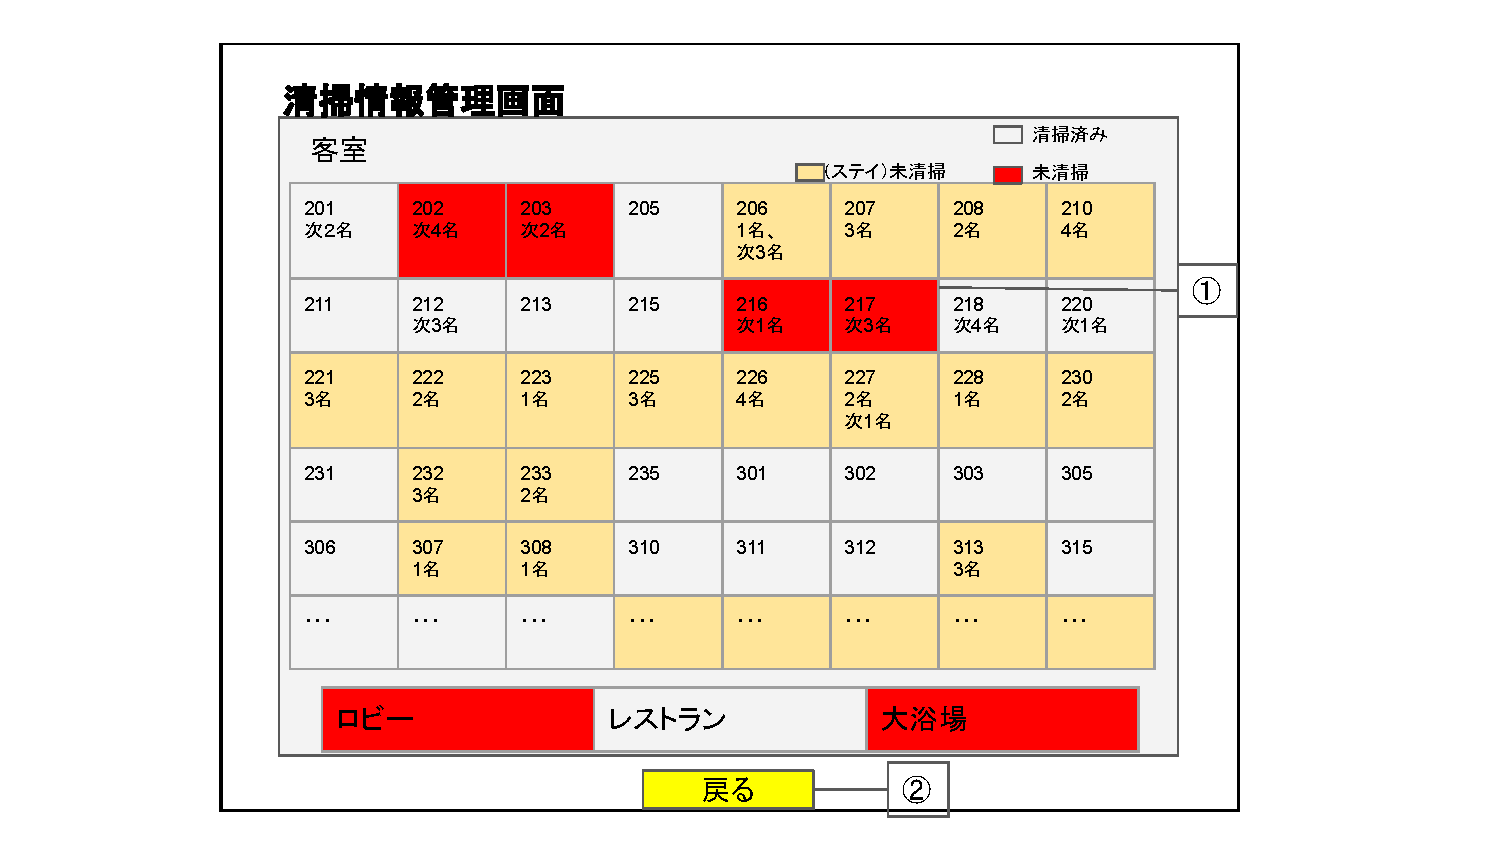
\includegraphics[width=150mm]{UI-seisou/user-seisouMain.pdf}
 \caption{清掃情報管理画面}
 \label{fig:seisou01}
\end{figure}

\begin{figure}[H]
 \centering
   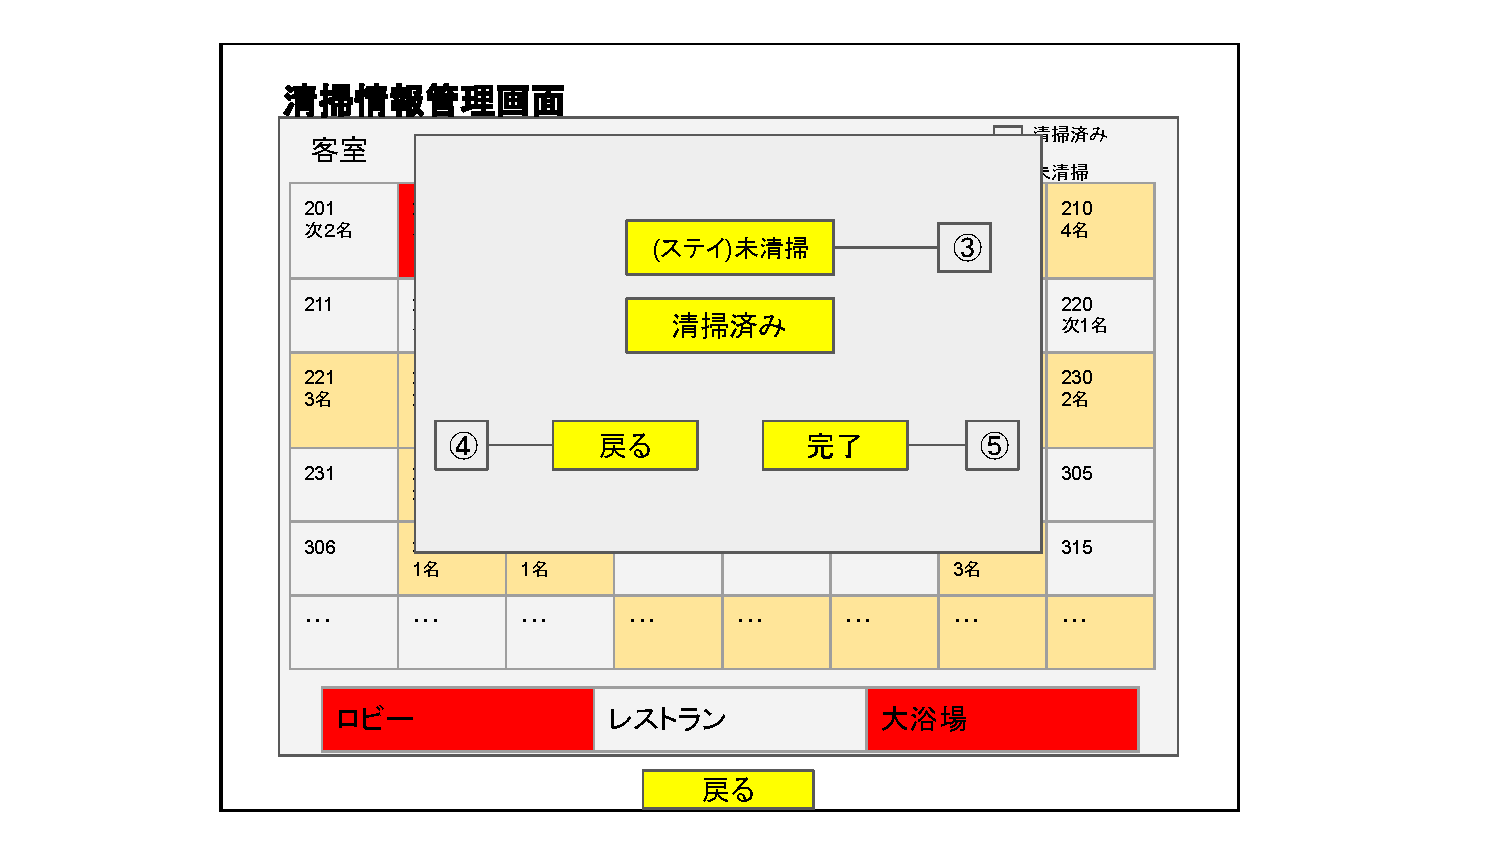
\includegraphics[width=150mm]{UI-seisou/user-cleaning01.pdf}
 \caption{清掃情報管理画面(ポップアップ表示)}
 \label{fig:seisou02}
\end{figure}


\begin{enumerate}
\renewcommand{\labelenumi}{\textcircled{\scriptsize \theenumi}}
\item 清掃情報変更\\ 赤と黄色の未清掃を押すことで,図\ref{fig:seisou02}に示すポップアップを表示する.
\item 戻る\\ 戻るを押すことで,図\ref{fig:TOP1}に示す総合TOP画面に遷移する.
\item 未清掃・清掃済みチェックボタン\\
未清掃,清掃済みへ変更する際に選択されるボタンである.
\item 戻る\\
戻るを押すことで,変更を反映せずにポップアップを消す.
\item 完了\\
完了を押すことでチェックボタンで選択したものを反映してポップアップを消す.
\end{enumerate}



\end{document}